\documentclass{beamer}
\usepackage{latexsym} 
\usepackage{graphicx}
\usetheme{Warsaw}

\title{Chapter 12}
\subtitle{Artificial Neural Networks}

\begin{document}
\maketitle

\begin{frame}
  \frametitle{Deep learning}
  \begin{itemize}
  \item Big in ML
  \item Set of algorithms to train neural networks
  \item Python libraries available
  \item Outline
    \begin{itemize}
    \item Forward propagation in ANNs
    \item Backpropagation to learn the parameters
    \item Debugging ANNs
    \item Alternative architectures (CNN, RNN)
    \end{itemize}
  \end{itemize}
\end{frame}

\begin{frame}
  \frametitle{Single neuron review}
  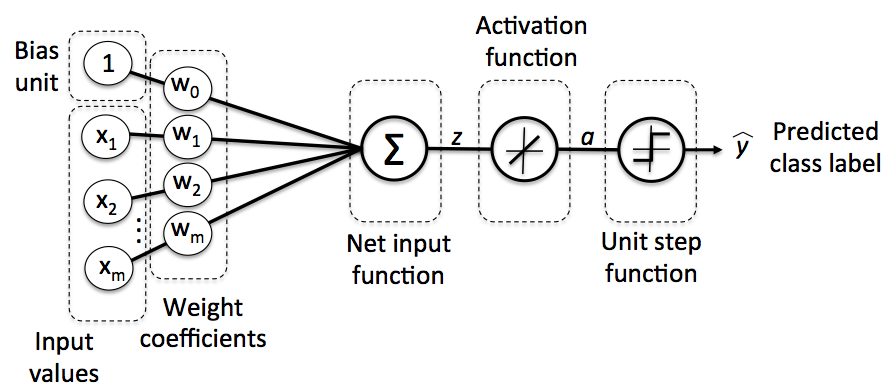
\includegraphics[width=\textwidth]{Code/ch12/images/12_01.png}  
\end{frame}

\begin{frame}
  \frametitle{Adaline review}
  \begin{itemize}
  \item Perceptron
    \begin{itemize}
    \item Update all weights, then recompute $\hat{y}$
    \item Weight update done after seeing each sample
      \[
      \Delta w_j = \eta \bigg( y^{(i)} - \hat{y}^{(i)} \bigg)x_{j}^{(i)}
      \]
    \end{itemize}
  \item Adaline
    \begin{itemize}
    \item Weight update done after entire training set has been seen
    \item In every epoch, update all weights as follows:
      \[
      \mathbf{w} := \mathbf{w} + \Delta \mathbf{w}, \quad \text{where } \Delta \mathbf{w} = - \eta \nabla J (\mathbf{w})
      \]
    \item I.e. compute the gradient based on all samples in the training set (this is known as batch gradient descent)
    \item SGD updates after seeing $n$ samples
    \item Mini-batch: middle ground bewteen SGD and batch GD
    \end{itemize}
  \end{itemize}
\end{frame}

\begin{frame}
  \frametitle{Weight update details}
  Partial derivative for each weight $w_j$ in the weight vector $\mathbf{w}$:
  \[
  \frac{\partial}{\partial w_j} J(\mathbf{w}) = \sum_i \big( y^{(i)} - a^{(i)} \big) x_{j}^{(i)}
  \]
  Here $y^{(i)}$ is the target class label of a particular sample $x^{(i)}$, and $a^{(i)}$ is the \textit{activation} of the neuron, which is a linear function in the case of Adaline: Remember that we defined the \textit{activation function} $\phi(\cdot)$ as follows:
  \[
  \phi(z) = z = a
  \]
  Here, the net input $z$  is a linear combination of the weights that are connecting the
  input to the output layer:
  \[
  z = \sum_j w_j x_j = \mathbf{w}^T \mathbf{x}
  \]
\end{frame}

\begin{frame}
  \frametitle{Multi-layer feedforward neural network}
  \center
  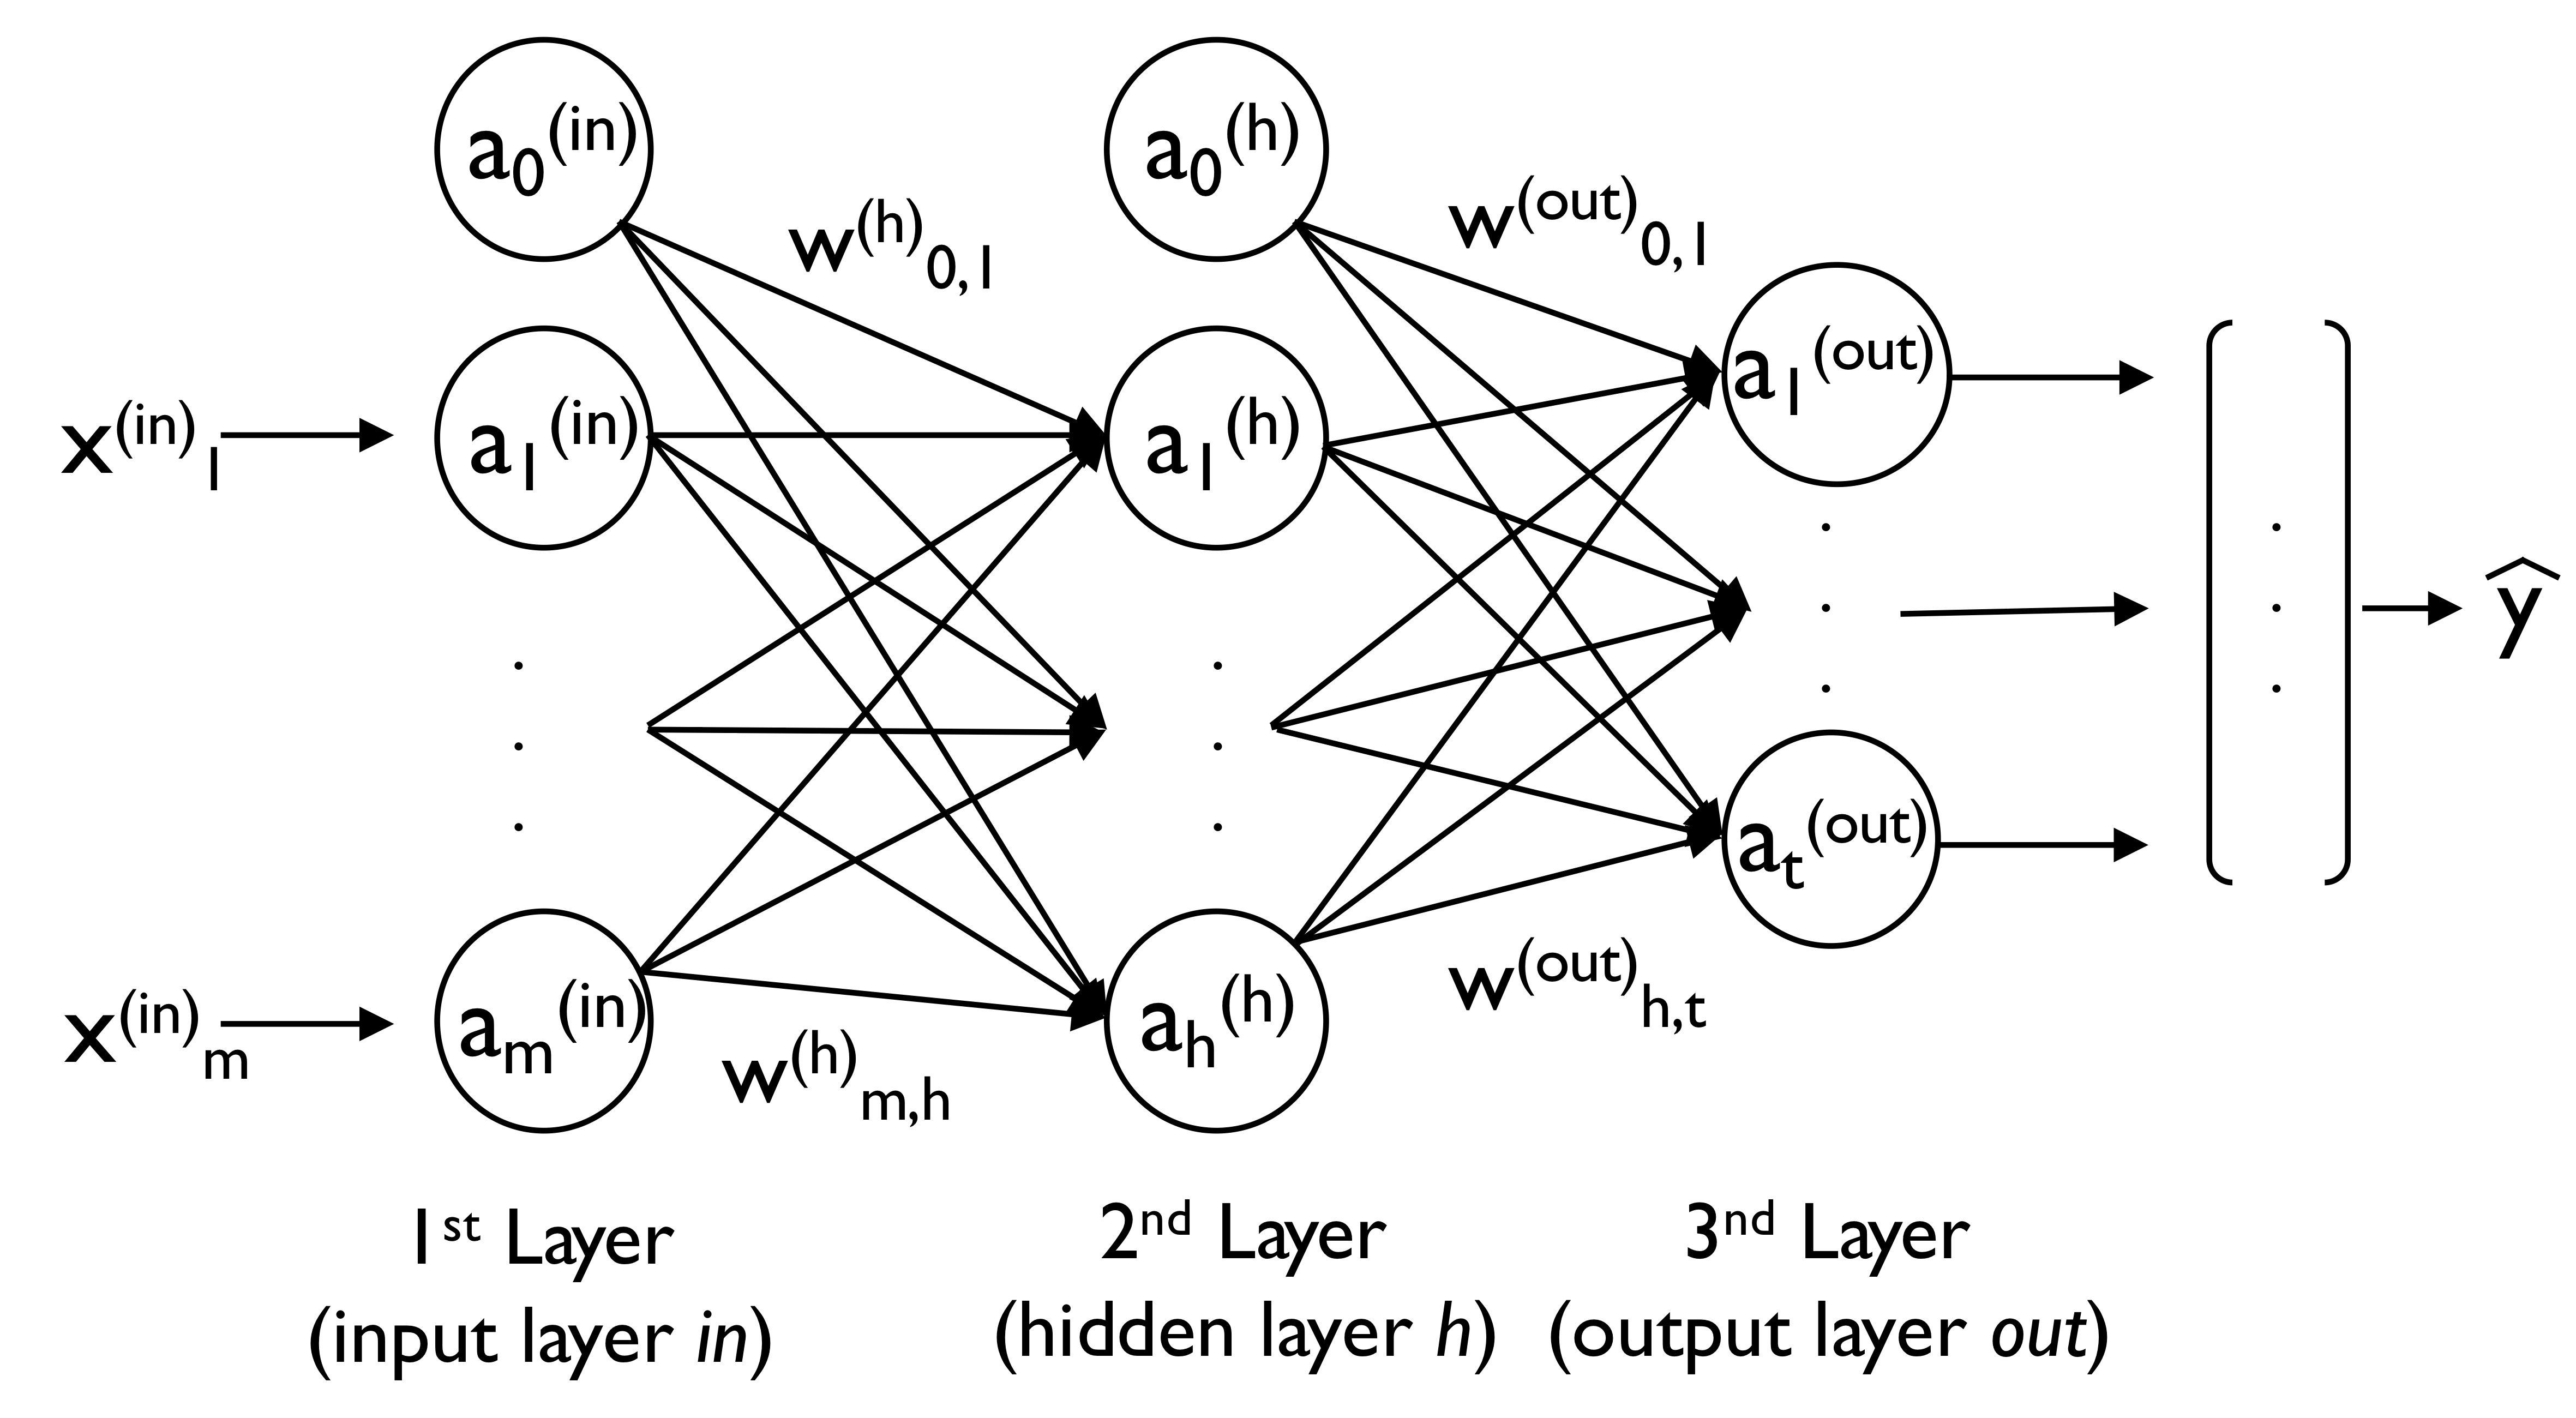
\includegraphics[scale=0.6]{Code/ch12/images/12_02.png}  
\end{frame}

\begin{frame}
  \frametitle{Notation}
  \begin{itemize}
  \item We denote the $i$th activation unit in the $l$th layer as $a_{i}^{(l)}$
  \item The activation units $a_{0}^{(1)}$ and $a_{0}^{(2)}$ are the \textit{bias units}, respectively, which we set equal to 1
  \item The activation of the units in the input layer:
    \[
    \mathbf{a}^{(i)} = 
    \begin{bmatrix}
      a_{0}^{(1)} \\
      a_{1}^{(1)} \\
      \vdots \\
      a_{m}^{(1)}
    \end{bmatrix}
    = 
    \begin{bmatrix}
      1 \\
      x_{1}^{(i)} \\
      \vdots \\
      x_{m}^{(i)}
    \end{bmatrix}
    \]
    \item The connection between the $k$th unit in layer $l$ to the $j$th unit in layer
    $l+1$ written as $w^{(l)}_{j, k}$
  \end{itemize}
\end{frame}

\begin{frame}
  \frametitle{Notation summary}
  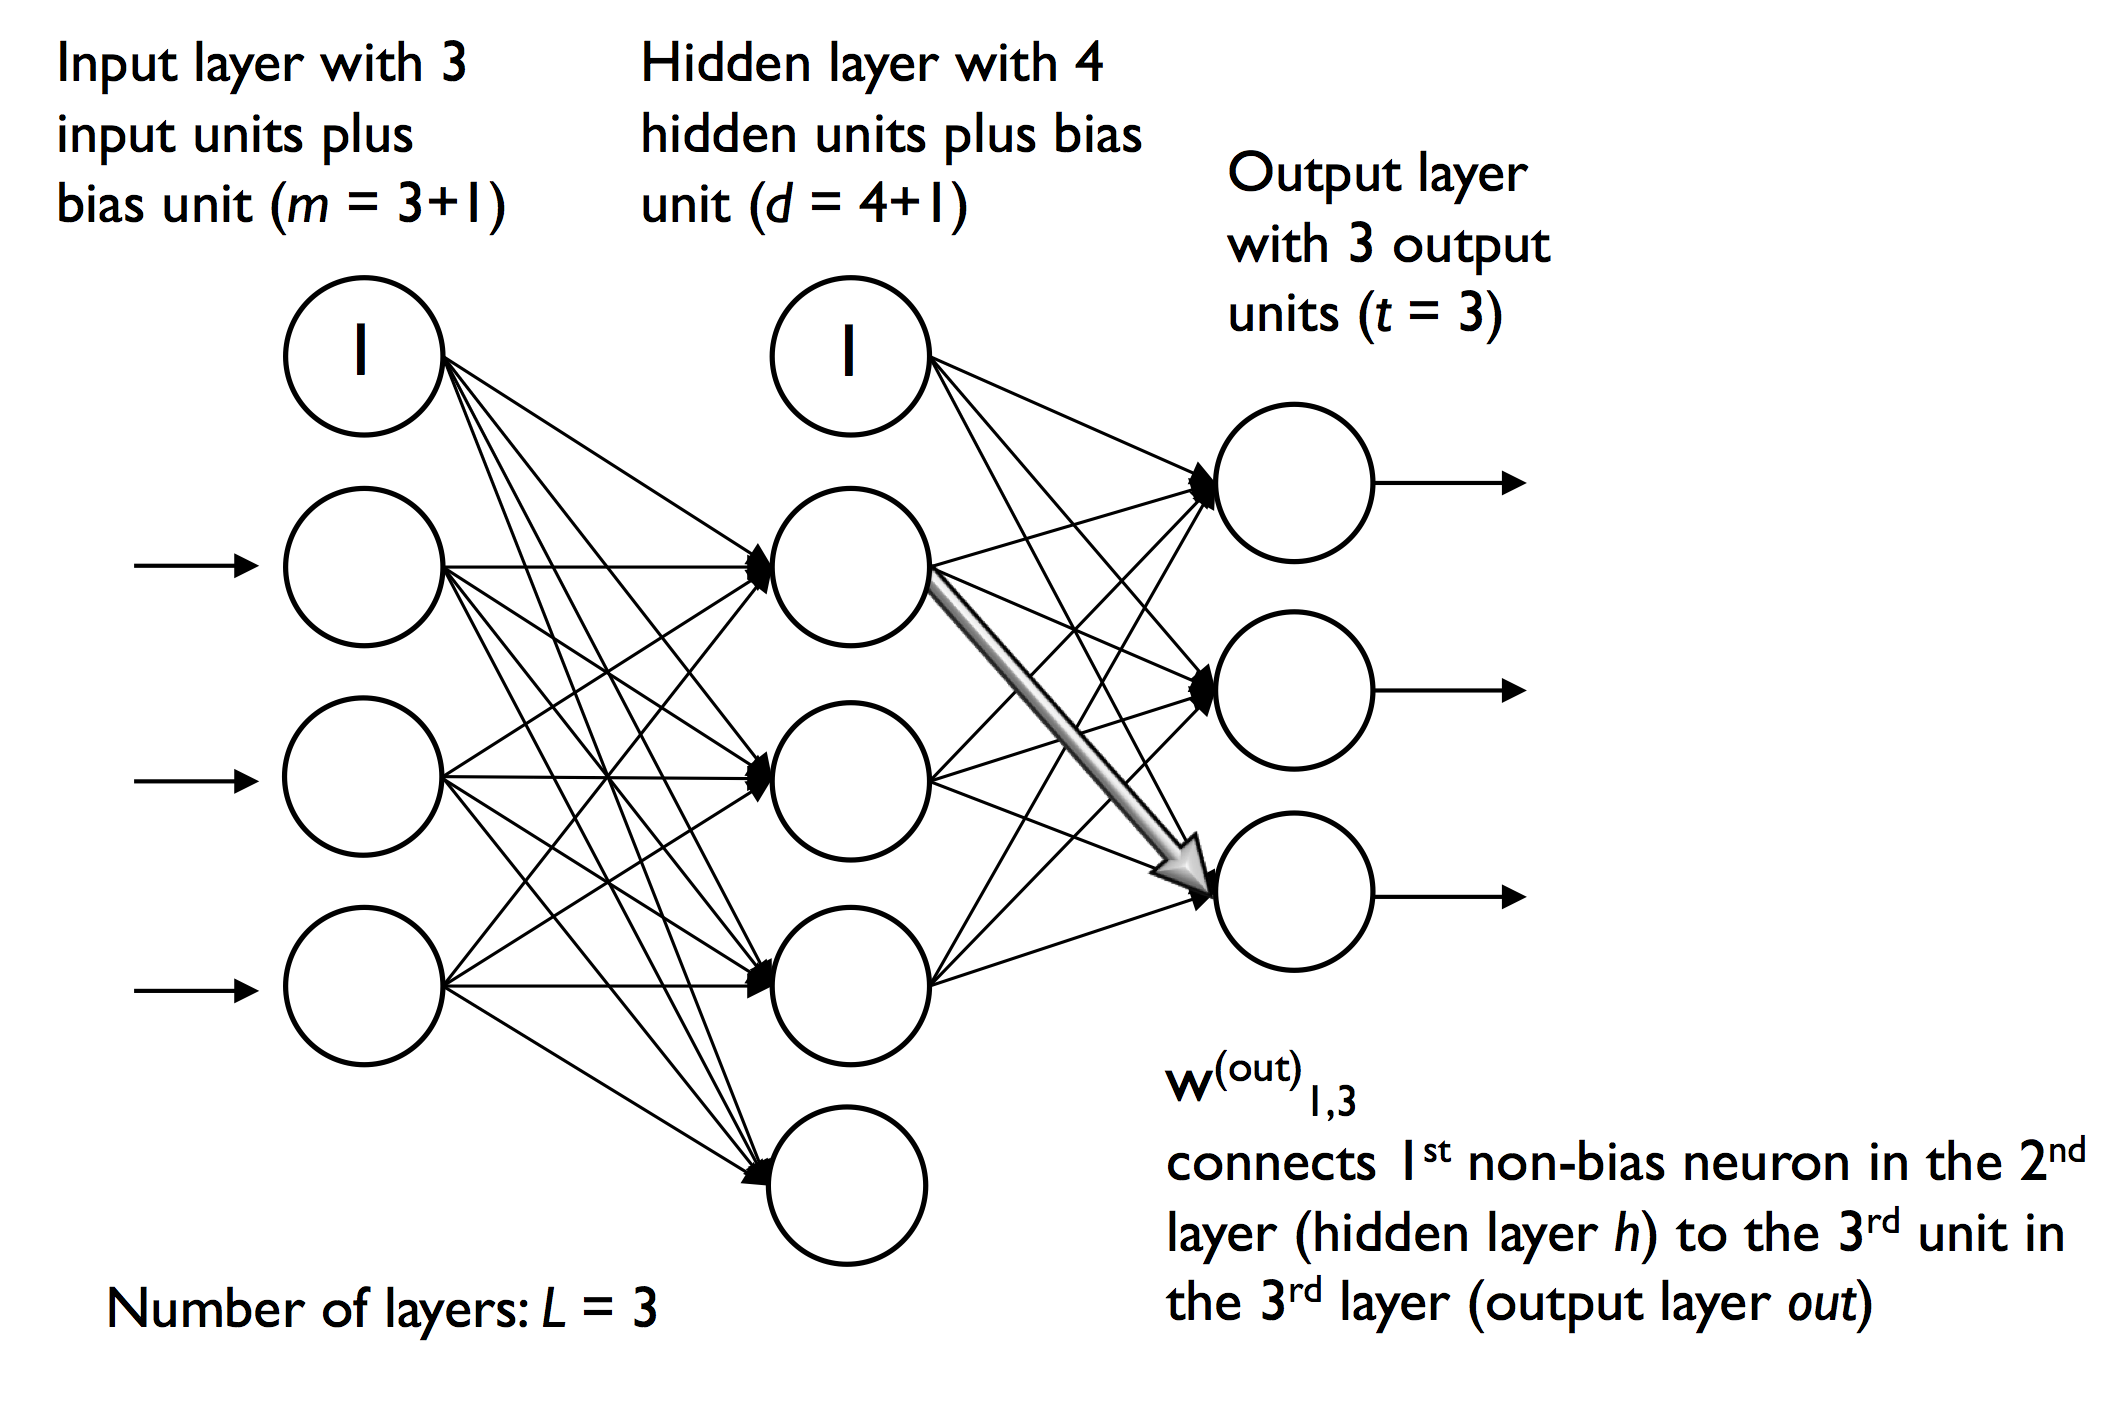
\includegraphics[scale=0.4]{Code/ch12/images/12_03.png}  
\end{frame}

\begin{frame}
  \frametitle{MLP learning procedure}
  \begin{enumerate}
  \item Starting at the input layer, forward propagate $\mathbf{x^{(i)}}$
  \item Calculate the error that we will want to minimize
  \item Find its derivative with respect to each weight
  \item Update the weights
  \end{enumerate}
\end{frame}

\begin{frame}
  \frametitle{Forward propagation}
  \begin{enumerate}
  \item Assume, input has $m$ dimensions
    \item Compute the net input $a_{1}^{(2)}$ for unit 1 in the hidden layer:
      \[
      z_{1}^{(2)} = a_{0}^{(1)} w_{1,0}^{(1)} + a_{1}^{(1)} w_{1, 1}^{(1)} + \dots + a_{m}^{(1)} w_{l, m}^{(1)}
      \]
    \item Compute the activation for unit 1 in the hidden layer:
      \[
      a_{1}^{(2)} = \phi \big( z_{1}^{(2)} \big)
      \]
    \item Here $\phi(\cdot)$ is the activation function
    \item Logistic sigmoid is often used:
      \[
      \phi(z) = \frac{1}{1 + e^{-z}}.
      \]
  \end{enumerate}
\end{frame}

\begin{frame}
  \frametitle{Sigmoid function}
  \center
  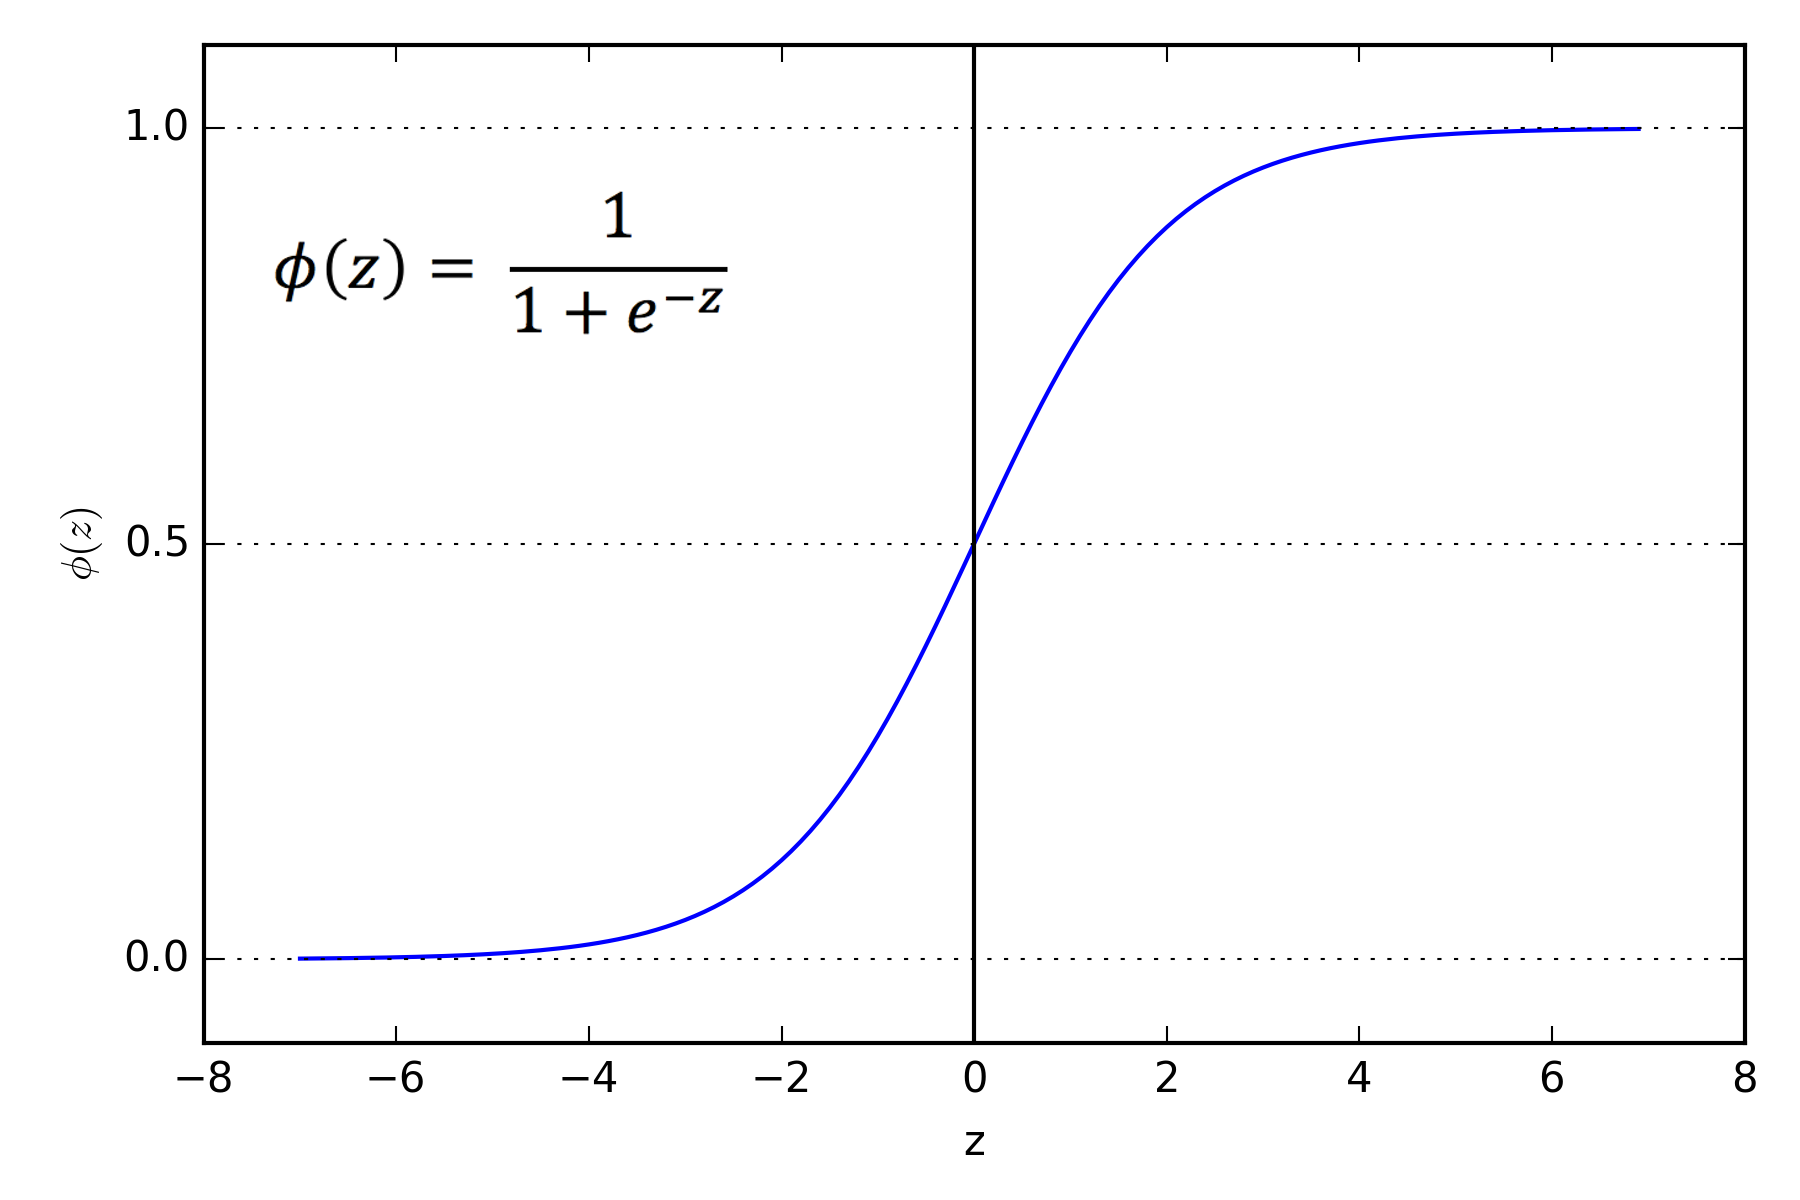
\includegraphics[scale=0.6]{Code/ch12/images/12_04.png}  
\end{frame}

\begin{frame}
  \frametitle{Vectorized notation}
  \begin{itemize}
  \item Write activation in a matrix form
  \item Readability + more efficient code
  \item Net inputs for the hidden layer:
    \[
    \mathbf{z}^{(2)} = \mathbf{W}^{(1)} \mathbf{a}^{(1)}
    \]
  \item Dimensions (ignoring bias units for simplicity)
    \[
    [h \times 1] = [h \times m] [m \times 1]
    \]
  \item Activations for the hidden layer:
    \[
    \mathbf{a}^{(2)} = \phi \big( \mathbf{z}^{(2)} \big)
    \]
  \end{itemize}
\end{frame}

\begin{frame}
  \frametitle{Matrix notation}
  \begin{itemize}
  \item Generalize computation to all $n$ samples in the training set
    \[
    \mathbf{Z}^{(2)} = \mathbf{W}^{(1)} \big[ \mathbf{A}^{(1)} \big]^T
    \]
  \item Matrix dimensions 
    \[
    [h \times n] = [h \times m] [n \times m]^T
    \]
  \item Activation matrix
    \[
    \mathbf{A}^{(2)} = \phi \big( \mathbf{Z}^{(2)}  \big)
    \]
    \item Now activation of the output layer
      \[
      \mathbf{Z}^{(3)} = \mathbf{W}^{(2)}  \mathbf{A}^{(2)} 
      \]
    \item Matrix dimensions
      \[
      [t \times n] = [t \times h] [h \times n]
      \]
    \item Output of the network
      \[
      \mathbf{A}^{(3)} = \phi \big( \mathbf{Z}^{(3)} \big), \; \mathbf{A}^{(3)} \in \mathbb{R}^{t \times n}.
      \]
  \end{itemize}
\end{frame}

\begin{frame}
  \frametitle{Cost function}
  The logistic Cost function is the same we used for logistic regression:
  \[
  J(\mathbf{w}) = -\sum_{i=1}^{n} y^{(i)} \log \big( a^{(i)} \big) + \big( 1 - y^{(i)} \big) \log \big( 1 - a^{(i)}\big)
  \]
  Here, $a^{(i)}$ is the sigmoid activation of the $i$th unit $a^{(i)} = \phi \big( z^{(i)} \big)$.
  Regularization:
  \[
  L2 = \lambda \lVert  \mathbf{w} \rVert^{2}_{2} = \lambda \sum_{j=1}^{m} w_{j}^{2}
  \]
  \[
  J(\mathbf{w}) = - \Bigg[ \sum_{i=1}^{n} y^{(i)} \log \big( a^{(i)} \big) + \big(1 - y^{(i)} \big) \log \big(1- a^{(i)} \big) \Bigg] + \frac{\lambda}{2} \lVert  \mathbf{w} \rVert^{2}_{2}
  \]

\end{frame}

\begin{frame}
  \frametitle{Cost function for all units in output layer}
  The activation of the third layer and the target class could be:
  \[
  a^{(3)} = 
  \begin{bmatrix}
    0.1 \\
    0.9 \\
    \vdots \\
    0.3
  \end{bmatrix}
  ,\; \mathbf{y} = 
  \begin{bmatrix}
    0 \\
    1 \\
    \vdots \\
    0
  \end{bmatrix}
  \]
  So, we need to generalize the logistic cost function to all activation units $j$ in our network. The cost function (without the regularization term) becomes:
  \[
  J(\mathbf{w}) = - \sum_{i=1}^{n} \sum_{j=1}^{t} y_{j}^{(i)} \log(a_{j}^{(i)}) + (1 - y_{j}^{(i)}) \log(1 - a^{(i)}_{j})
  \]
  Superscript $i$ is the index of a particular sample in training set
\end{frame}

\begin{frame}
  \frametitle{Cost function for the entire network}
  Sum all the weights in the entire network in the regularization term:
  \[
  J(\mathbf{w}) = - \Bigg[ \sum_{i=1}^{n} \sum_{j=1}^{m} y_{j}^{(i)}  \log \bigg( \phi \Big( z_{j}^{(i)} \Big) \bigg) + \Big(1 - y_{j}^{(i)} \Big) \log  \bigg(1 - \phi \Big( z_{j}^{(i)} \Big)  \bigg) \Bigg] +
  \]
  \[
  + \frac{\lambda}{2} \sum_{l=1}^{L-1} \sum_{i=1}^{u_l} \sum_{j=1}^{u_{l+1}} \Big(w_{j, i}^{(l)}\Big)^2
  \]
  The following expression represents the L2-penalty term:
  \[
  \frac{\lambda}{2} \sum_{l=1}^{L-1} \sum_{i=1}^{u_l} \sum_{j=1}^{u_{l+1}} \Big(w_{j, i}^{(l)}\Big)^2
  \]
\end{frame}

\begin{frame}
  \frametitle{Minimizing the cost function}
  We want to minimize the cost function $J(\mathbf{w})$, so we calculate the partial derivative with respect to each weight for every layer in the network:
  \[
  \frac{\partial J(\mathbf{W})}{\partial w_{j, i}^{(l)}}
  \]
\end{frame}

\begin{frame}
  \frametitle{}
  \begin{itemize}
  \item
  \end{itemize}
\end{frame}

\begin{frame}
  \frametitle{}
  \begin{itemize}
  \item
  \end{itemize}
\end{frame}

\begin{frame}
  \frametitle{}
  \begin{itemize}
  \item
  \end{itemize}
\end{frame}

\begin{frame}
  \frametitle{}
  \begin{itemize}
  \item
  \end{itemize}
\end{frame}

\begin{frame}
  \frametitle{}
  \begin{itemize}
  \item
  \end{itemize}
\end{frame}

\begin{frame}
  \frametitle{}
  \begin{itemize}
  \item
  \end{itemize}
\end{frame}

\begin{frame}
  \frametitle{}
  \begin{itemize}
  \item
  \end{itemize}
\end{frame}

\end{document}
